\section{实体对齐方法}
\label{sec:3_entity_extraction}
% 我们需要的是什么样的视觉特征,以及为什么
本章所提方法是针对名词短语或名词融合图片中的视觉信息。也有相关工作尝试以词为粒度融合视觉信息,例如文献\cite{20_wu-etal-2021-good,22_li-etal-2021-vision}均采用了门控机制来控制图片的全局特征与输入序列中每个单词的隐层表示的融合。然而,这种方式为模型所提供的图片信息依旧是不明确的。为此,我们选择将图片中与名词或短语相对应的视觉目标提取出来再进行信息的融合。该过程涉及到如何将句子中的名词或短语与图片中的视觉目标对齐。图\ref{fig:3_entity_extraction}为本文的解决方案。
\begin{figure}[!htbp]
    \centering
    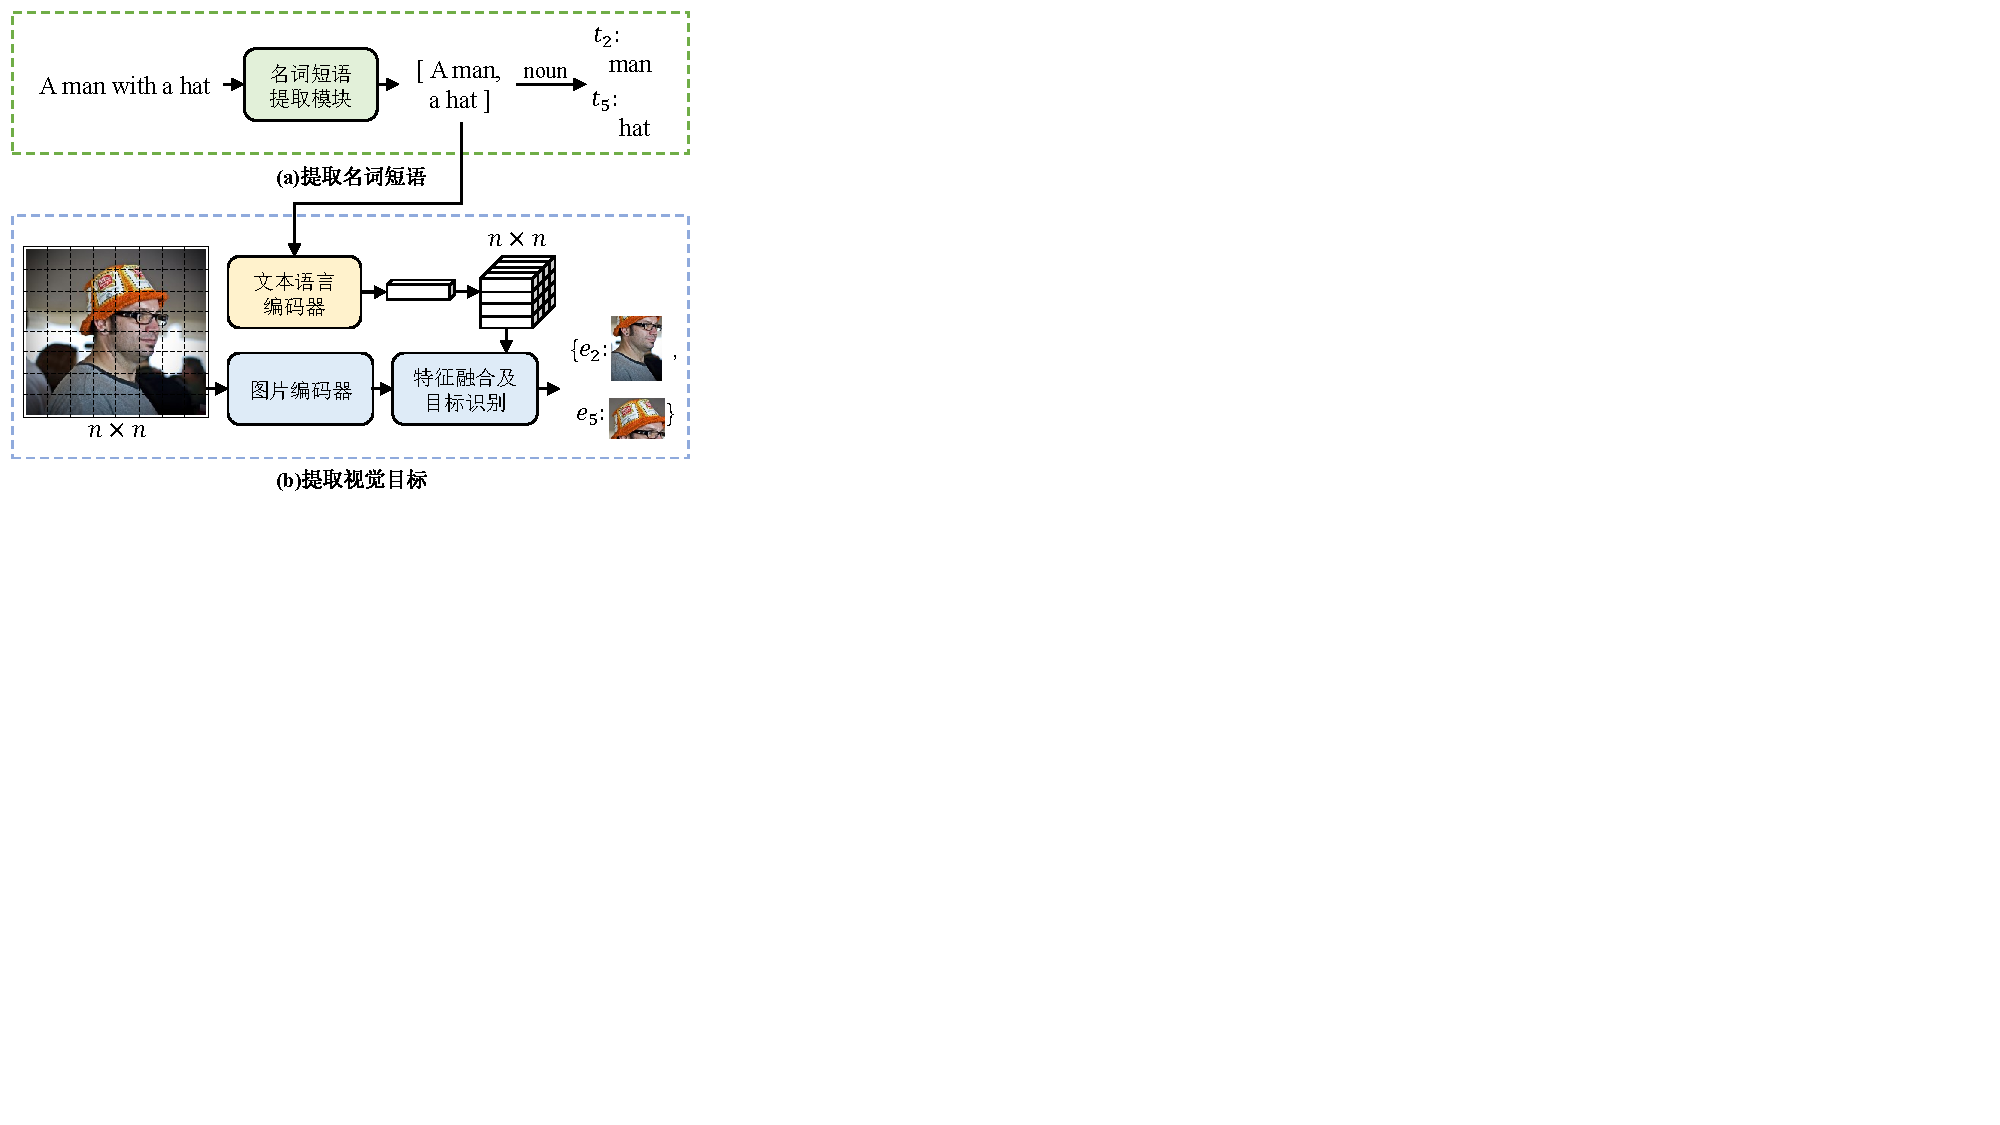
\includegraphics{Img/fig_3_entity_extraction.pdf}
    \bicaption{实体提取与对齐方法}{Entity extraction and alignment methods}
    \label{fig:3_entity_extraction}
\end{figure}

图\ref{fig:3_entity_extraction}a展示了名词短语的提取过程。本文采用成熟的spaCy\footnote{https://spacy.io/}工具提取源语言句子中的名词短语。这样再通过对句子的词性标注即可获得所提取的短语中的名词。例如,将句子“A man with a hat.”输入到短语提取工具中,可得到名词短语“A man”和“a hat”,其中“man”和“hat”就是本文需要的名词。因为考虑到句子中仅名词或名词短语在图片中有着直接对应的视觉目标,所以在该方法中不考虑源语言句子中其它类型的短语。

图\ref{fig:3_entity_extraction}b展示了图片中视觉特征的提取过程。在得到了文本中的名词短语后,就可以根据这些短语提取图片中对应的区域作为视觉目标。为此,本文采用了文献\cite{24_DBLP:conf/iccv/YangGWHYL19}提出的单步视觉目标提取法(one-stage visual grounding)。该方法的输入是一张图片和一个短语,模型的输出为短语所对应的图片区域。简化工作流程为,利用预训练的语言模型(如BERT\cite{25_DBLP:conf/naacl/DevlinCLT19})和预训练的图片编码器(如Darknet-53\cite{26_DBLP:journals/corr/abs-1804-02767})分别为短语和图片提取语义特征向量和图片栅格特征,然后将语义特征向量与栅格特征中每个栅格的特征相融合(如拼接)。将融合的特征送入检测模块判断栅格中哪些位置是属于输入的短语,最后拼接成一块完整的区域。例如,将“A man”和完整的图片输入到模型中,提取出来的就是图片中“男人”所对应的区域。

经过以上过程,就可得到源语言句子中的名词、名词短语、视觉目标以及它们之间的对应关系。